\graphicspath{{notes/asy/}}
\thispagestyle{empty}

\title{Math 120A --- Introduction to Group Theory}
\author{Neil Donaldson}
\date{Fall 2018}
\maketitle 

\subsection*{Text}
\begin{itemize}
\item \emph{An Introduction to Abstract Algebra}, John Fraleigh, 7th Ed 2003, Adison--Wesley (optional).
\item Also check the library for entries under ``Group Theory" and ``(Abstract) Algebra". There have been a plethora of textbooks written for Undergraduate group theory courses and the first few chapters of most of them will cover similar ground to the core text. 
\end{itemize}

\section{Introduction: what is abstract algebra and why study groups?}

To be \emph{abstract} is to remove context and application and study the \emph{structure} of something. Abstract mathematics essentially involves studying the patterns and symmetries inherent in the real world from an abstract viewpoint so as to see the commonalities between structures in seemingly distinct places: we shall see an example of a common structure shortly.\\

A \emph{group} is one of the simplest algebraic structures. This in itself is a good reason to study groups: they are (relatively) easy! Indeed you have been working with groups for years: a group is a set with one operation (like the real numbers $\R$ with $+$) that has a small number of additional properties.\footnote{You are already familiar with objects far more complicated than this (e.g. $\R$ with the two operations $+,\cdot$ is a \emph{field}, $(\R^n,+,\cdot)$ is a \emph{vector space},  the set of equivalence classes modulo six $(\Z_6,+_6,\cdot_6)$ is a \emph{ring}.} Since there is only one operation, the number of options is very limited. Sometimes \emph{doing the only thing you can} will lead you to a correct proof!\\

The real reason to study groups is that they have wide applications. For instance:

\begin{description}
\item[Geometry] A large part of modern Geometry involves the study of groups --- surfaces, polyhedra, the set of lines in a vector space --- these sets have many different groups associated to them which help the geometer describe and classify them.
\item[Combinatorics] When studying collections of objects, groups of permutations (reorderings) of sets are widely used.
\item[Galois Theory] Groups describe symmetries in the roots of polynomial equations.
\item[Chemistry] Groups are used to describe the symmetries of molecules and of crystalline substances.
\item[Physics] Materials science sees group theory similarly to Chemistry, while modern theories of the nature of the Universe (e.g.\ string theory) rely heavily on groups.
\end{description}


\subsection*{Motivational example}\hypertarget{sec:motiv}{}

What do an equilateral triangle and an arbitrary collection $\{1,2,3\}$ of three objects have in common? The obvious answer is the number \emph{three,} but we can say a lot more. Both objects have \emph{symmetries}: rotations and reflections of the triangle and permutations of the set $\{1,2,3\}$. Considering \emph{compositions} of these symmetries, we will see that they are essentially the \emph{same}.

\paragraph{Permuations of $\{1,2,3\}$} These can be written in \emph{cycle notation}:\footnote{We will return to this notation later so don't feel you have to be an expert on it now. The permutation $(12)$ is known as a \emph{2-cycle} because it permutes two objects. The permutation $(123)$ is similarly referred to as a \emph{3-cycle.}} for example, the cycle $(12)$ represents swapping 1 and 2 and leaving 3 alone. For instance, as functions,
\[(12):\begin{cases}
1\mapsto 2\\
2\mapsto 1\\
3\mapsto 3
\end{cases}\qquad\text{and}\qquad
(123):\begin{cases}
1\mapsto 2\\
2\mapsto 3\\
3\mapsto 1
\end{cases}\]
It is not hard to convince yourself that there are six distinct permutations of $\{1,2,3\}$: for brevity, we will use the symbols $e,\mu_1,\mu_2,\mu_3,\rho_1,\rho_2$.
\[\begin{array}{c|c|c}
\text{Identity: leave everything alone} & \text{Swap two numbers} & \text{Permute all three}\\\hline
e=() & \mu_1=(23) & \rho_1=(123)\\
& \mu_2=(13) & \rho_2=(132)\\
& \mu_3=(12) &
\end{array}\]
We can compose these permutations. For instance
\[\mu_1\circ\rho_2=(23)(132):\begin{cases}
1\mapsto 3\mapsto 2\\
2\mapsto 1\mapsto 1\\
3\mapsto 2\mapsto 3
\end{cases}\]
The result is the same as that obtained by the permutation $(12)=\mu_3$, whence we write
\[\mu_1\circ\rho_2=\mu_3\]
The full list of compositions of the symmetries is shown in the following table: read the left column first, then the top row: our previous calculation is shown in red.\label{intro:table}
\[\begin{array}{c||c|c|c|c|c|c}
\circ & e & \rho_1 & \textcolor{red}{\rho_2} & \mu_1 & \mu_2 & \mu_3\\
 \hline\hline
e & e & \rho_1 & \rho_2 & \mu_1 & \mu_2 & \mu_3\\
\hline
\rho_1 & \rho_1 & \rho_2 & e & \mu_3 & \mu_1 & \mu_2\\
\hline
\rho_2 & \rho_2 & e & \rho_1 & \mu_2 & \mu_3 & \mu_1\\
\hline
\textcolor{red}{\mu_1} & \mu_1 & \mu_2 & \textcolor{red}{\mu_3} & e & \rho_1 & \rho_2\\
\hline
\mu_2 & \mu_2 & \mu_3 & \mu_1 & \rho_2 & e & \rho_1\\
\hline
\mu_3 & \mu_3 & \mu_1 & \mu_2 & \rho_1 & \rho_2 & e
\end{array}\]


\begin{minipage}{0.6\textwidth}
\paragraph{The Equilateral Triangle}
What does all this have to do with a triangle? If we label the vertices of an equilateral triangle 1,2,3, then the above permutations correspond to symmetries of the triangle: $\rho_1$ and $\rho_2$ are rotations, while each $\mu_i$ performs a reflection in the altitude through the vertex $i$. The two sets of symmetries apply to different objects, but their interactions are identical.\\

One might obtain intuition about the permutations of $\{1,2,3\}$ by viewing them as symmetries of a triangle. In particular, there is a qualitative difference between the \emph{rotations} $\rho_1,\rho_2$ and the \emph{reflections} $\mu_1,\mu_2,\mu_3$. That composition of reflections produces a rotation is clear in the triangle setting. That composition of 2-cycles makes a 3-cycle is not so clear.
\end{minipage}\begin{minipage}{0.4\textwidth}
\flushright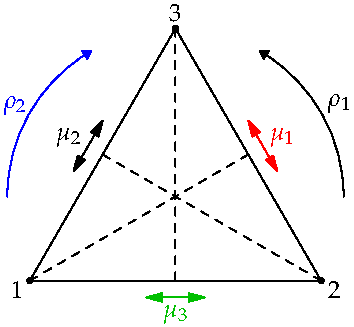
\includegraphics{intro-s3}
\end{minipage}\\[8pt]


Group theory is about ideas like this: in group theory the symmetries and patterns associated to objects are more important than the objects themselves and can lead to unexpected connections. In this introduction we considered two groups:
\begin{description}
	\item[$S_3$:] the \emph{symmetric group} on three letters/permutations of $\{1,2,3\}$.
	\item[$D_3$:] the \emph{dihedral group} of order six/symmetries of the equilateral triangle.
\end{description}
The fact that the resulting structures are identical will be written $S_3\cong D_3$, and we will say that these groups are \emph{isomorphic.}\footnote{We will explain the term \emph{isomorphic} more concretely later on and revisit both examples. Also observe that was use the congruence symbol $\cong$ to denote isomorphic groups: you should think about why this makes sense\ldots} 


\section{Binary operations}\hypertarget{sec:binary}{}

A group is essentially a set with a single operation that allows us to combine two elements of the set to create a new element. We start by formally defining such operations.

\begin{defn}
A \emph{binary operation} $*$ on a set $X$ is a function $*:X\times X\to X$ which is \emph{defined for all} pairs of elements in $X$. We say that $X$ is \emph{closed under $*$.} Otherwise said
\[\forall x_1,x_2\in X,\ x_1*x_2\in X\] 
\end{defn}

\paragraph{Examples}
\begin{enumerate}
	\item Addition $+$ and multiplication $\cdot$ are binary operations on any of the usual sets of numbers: $\N$, $\R$, $\C$, $\Q$, $\Z$, $\R^+$, $\Q^+$, etc.
	\item The sets $\R,\Q,\C,\Z$ with $*$ being subtraction.
	\item Any vector space (e.g.\ $\R^n$ or $\C^n$) has addition as a binary operation.
	\item $\R^3$ with cross/vector product $\times$.
	\item $\{\text{Functions } f:V\to V\}$, where $V$ is any set and $*=\circ$ (composition of functions).
	\item $\C$ with $*$ the Hermitian product: $z*w=z \cl w$.
	\item $\N=\Z^+$ with $*$ the least common multiple: e.g.\ $4*10=20$.
	\item $\N$ with $*$ the largest common prime factor: e.g.\ $65*20=5$.
	\item The set $A=\{0,1,2,3\}$ with $a*b=ab \mod 4$ (i.e.\ the remainder upon dividing $ab$ by 4).
\end{enumerate}

There is no requirement that a binary operation be surjective (i.e.\ $X*X$ need not be all of $X$; see example 1 where the image of $+$ on $\N$ is always $\ge 2$).

\subsubsection*{(Multipliction) Tables}

Binary operations on finite sets can be written in tabular form.\footnote{For abstract operations these are often written multiplicatively, and are therefore known as \emph{multiplication tables.}} For instance, example 9 above can be written
\[\begin{array}{c||c|c|c|c}
* & 0 & 1 & 2 & 3\\
\hline\hline 0 & 0 & 0 & 0 & 0\\
\hline 1 & 0 & 1 & 2 & 3\\
\hline 2 & 0 & 2 & 0 & 2\\
\hline 3 & 0 & 3 & 2 & 1
  \end{array}\quad\text{ where we find $a*b$ by taking $a$ in the left column and $b$ along the top.}\]
Compare with the operation table on page \pageref{intro:table}. It would not be sensible to use a table to describe the other examples of binary operations since all the other sets are infinite. 

\subsubsection*{Non-examples}

Here are two non-examples of binary operations:
\begin{enumerate}
  \item $(\Q,*)$ with $a*b=\frac ab$ is not a binary operation since $a*0$ is undefined for all $a$.
  \item Let $\mathcal M=\{2\times 2\text{ matrices with determinant 7}\}$ with $A*B=AB$ being matrix multiplication. Since $\det(AB)=\det A\det B$,
  it follows that $\det(A*B)=49$ and so $A*B\not\in\mathcal M$. Thus $*$ is not a binary operation on $\mathcal M$.
\end{enumerate}

\subsubsection*{Subsets and binary operations}

It is common to consider whether subsets are closed under a given binary operation. For instance:

\begin{enumerate}
	\item The negative integers $\Z^-$ are closed under addition but not multiplication. As a little revision of quantifier notation, let us examine these claims carefully:
	\begin{itemize}
	  \item That $\Z^-$ is closed under addition can be written $\forall x,y\in\Z^-,\ x+y\in\Z^-$. This is trivial to prove:\\
	  Given $x,y\in\Z^-$ we have $x,y<0\implies x+y<0\implies x+y\in\Z^-$.
	  \item That $\Z^-$ is not closed under multiplication means that $\forall x,y\in\Z^-,\ xy\in\Z^-$ is \emph{false.} Recalling the negation of quantified statements, this is equivalent to
	  \[\exists x,y\in\Z^-\ \text{such that}\ xy\not\in\Z^-\]
	  This is also trivial to prove: the example $x=y=-1\implies xy=1$ suffices.
	\end{itemize}
	\item\label{intro:modex} Let $Y\subseteq\Z$ be the set of integers whose remainder is 1 when divided by 3: i.e.
	\[Y=3\Z+1=\{x\in\Z:x\equiv 1\mod 3\}=\{1,4,7,10,13,\ldots, -2,-5,-8,\ldots\}\] Is $Y$ 	closed under $+$? Or $\cdot$?
	\begin{itemize}
	  \item Under addition: not closed. For example 1 and 4 both lie in $Y$, yet $1+4=5\not\in Y$.
	  \item Under multiplication: closed. Simply observe that
	  \[(1+3n)(1+3m)=1+3n+3m+9mn=1+3(m+n+3mn)\]
	  has remainder 1 on division by 3 and thus lies in $Y$.
	\end{itemize}
	Note that we proved the following quantified statements:
	\begin{itemize}
	  \item $\exists x,y\in Y$ such that $x+y\not\in Y$.
	  \item $\forall x,y\in Y$ we have $xy\in Y$.
	\end{itemize}
\end{enumerate}

\subsubsection*{Associativity and Commutativity}

We introduce two important properties that might be satisfied by a binary operation.

\begin{defn}
A binary operation $*$ on a set $X$ is:
\begin{description}
\item[Associative] if $\forall a,b,c\in X$, we have $a*(b*c)=(a*b)*c$.
\item[Commutative] if $\forall a,b\in X$, we have $a*b=b*a$.
\end{description}
\end{defn}

If $*$ is associative then writing $a_1*a_2*\cdots *a_n$ is unambiguous. The fact that we can do this without using brackets makes associativity a highly desirous property! Examples 1, 3, 5, 7, 8, 9 in the first list in this section are associative. Examples 1, 3, 7, 8, 9 are commutative.




% \subsubsection*{Notation: additive and multiplicative structures}
% 
% Some algebraists use $+$ to denote a commutative binary operation, regardless of whether the operation is somehow derived from the `usual' addition of numbers.  A binary operation is often described as \emph{additive} if the operation is written $+$, and \emph{multiplicative} if the operation is written using juxtaposition ($a\ast b=ab$).\\
% The choice of whether to write a group additively or multiplicatively is largely one of style, not substance.\\

The table of a commutative binary operation necessarily has \emph{diagonal symmetry.} For example our earlier table is symmetric about the principal diagonal $\searrow$. Conversely, non-commutative operations must have non-symmetric tables.\\
\begin{gather*}\label{eq:commute}
\begin{array}{ccc}
  \begin{array}{c||c|c|c|c}
* & 0 & 1 & 2 & 3\\
\hline\hline 0 & 0 & 0 & 0 & 0\\
\hline 1 & 0 & 1 & 2 & 3\\
\hline 2 & 0 & 2 & 0 & 2\\
\hline 3 & 0 & 3 & 2 & 1
  \end{array}
   &&
\begin{array}{c||c|c|c|c}
* & a & b & c & d\\
\hline\hline a & d & c & d & c\\
\hline b & a & b & a & d\\
\hline c & a & c & a & b\\
\hline d & c & c & a & c
  \end{array}\\
&&\\
\text{A commutative operation (ex 9)}&\hspace*{1cm}&\text{A non-commutative operation}
  \end{array}
\end{gather*}
Indeed the second table is not associative, for $(a*b)*c=c*c=a$ while $a*(b*c)=a*a=d$.

\subsubsection*{Demonstrating Associativity}

If you want to demonstrate the associativity of a binary operation on a set with $n$ elements, then it looks like you might have to check the equation $x*(y*z)=(x*y)*z$ for $n^3$ separate cases! This will likely prove extremely tedious. Instead, there are two standard ways of demonstrating associativity. The first is very easy, while the second requires a little thought to use.

\begin{description}
\item[By Restriction] If a binary operation $*$ on $X$ is associative, then $*$ is automatically associative when restricted to any subset $Y\subseteq X$. For example, multiplication of integers is associative, whence multiplication is also associative on the set $Y=3\Z+1$ as considered on page \pageref{intro:modex}.
\item[Functional Composition] The idea is to recognize a binary operation as some form of functional composition. This might be very easy, or more difficult. The key result is as follows.
\end{description}

\begin{thm}\label{thm:funcassoc}
Let $V$ be any set. Composition of functions $f:V\to V$ is associative.\\
If $V$ has at least 2 elements, then composition is non-commutative.
\end{thm}

\begin{proof}
We first need to prove that for all functions $f,g,h:V\to V$ we have $(f\circ g)\circ h=f\circ(g\circ h)$. Two functions are equal if and only if they do the same thing to every element $x\in V$. Now
\begin{gather*}
((f\circ g)\circ h)(x)=(f\circ g)(h(x))=f(g(h(x)))\quad\text{and,}\\
(f\circ(g\circ h))(x)=f((g\circ h)(x))=f(g(h(x)))
\end{gather*}
Thus $\circ$ is associative. Showing non-commutativity is an exercise\ldots
%  To see that $\circ$ is non-commutative we have to exhibit a counter-example for \emph{any} $V$ with at least two elements. Let $a\neq b$ be two elements in $V$ and define  $f,g:V\to V$ by $f(x)=a,\ g(x)=b,\ \forall x\in V$. Then,
% \[f\circ g:x\mapsto f(b)=a,\qquad g\circ f:x\mapsto g(a)=b.\]
% $\circ$ is therefore non-commutative.
\end{proof}

For a first example of the Theorem, return to the introduction: the symmetries of an equilateral triangle may be viewed as a collection of six functions mapping the set of corners of the triangle $V=\{1,2,3\}$ to itself. The binary operation is functional composition and is thus associative.\\

In practice, one may need to do more work, as the following general example shows.

\begin{cor}\label{cor:assoc}
Matrix multiplication of square matrices is associative and non-commutative.
\end{cor}

You should have done the relevant work in a basic linear algebra course: in the presence of a basis, matrix multiplication by a square matrix corresponds to the action of a linear map on a vector space. For example, if $V=\R^2$, then the square matrix $A=\begin{smatrix}
	1&3\\
	2&-1
	\end{smatrix}$ describes a linear map $L_A:\R^2\to\R^2$ by
	\[L_A:\twovec xy\mapsto\begin{pmatrix}
	1&3\\
	2&-1
	\end{pmatrix}\twovec xy=\twovec{x+3y}{2x-y}\]
	Conversely, the linear map define by
	\[L_B:\twovec xy\mapsto \twovec{2x+7y}{-x+3y}\]
	has matrix $B=\begin{smatrix}
	2&7\\
	-1&3
	\end{smatrix}$. The matrix of the linear map $L_A\circ L_B$ is precisely the matrix $AB$. In this way, matrix multiplication of $2\times 2$ real matrices, corresponds precisely to the composition of linear maps on $\R^2$. The correspondence holds in general,\footnote{If $\cB=\{\vect en\}$ is a basis of a vector field $V$ over a field $\F$, then a linear map $L:V\to V$ has matrix
	\[[L]=(L(\ve_1)\cdots L(\ve_n))\]
	with $j^\text{th}$ column $L(\ve_j)$. If $L_1,L_2$ are linear maps then $[L_1\circ L_2]=[L_1]\circ[L_2]$. You will prove this in linear algebra if you haven't already done so.} hence the result.
% 
% \begin{proof}
% You should have verified the following in a basic linear algebra course. Suppose that $V$ is an $n$-dimensional vector space over a field $\F$ with basis $\cB=\{\vect en\}$. There is a bijective correspondence between the set of $n\times n$ matrices $M_n(\F)$ with entries in $\F$, and the set of linear maps
% \[\cL(V)=\bigl\{L:V\to V\bigm| \forall a,b\in\F,\vv,\vw\in V,\ L(a\vv+b\vw)=aL(\vv)+bL(\vw)\bigr\}\]
% from $V$ to itself. The correspondence is as follows:
% \begin{itemize}
%   \item If $A\in M_n(\F)$, define $L_A\in\cL(V)$ by $L_A(\vx)=A\vx$.
%   \item If $L\in\cL(V)$, define the matrix $A=[L]$ such that its $j^\text{th}$ column is the vector $L(\ve_j)$.
% \end{itemize}
% A little work shows that the matrix of the composition of two linear maps is given by the product of the corresponding matrices
% \[[L_A\circ L_B]=[L_A][L_B]=AB\]
% Armed with this information, matrix multiplication is simply composition of functions in disguise and its associativity follows immediately from Theorem \ref{thm:funcassoc}.
% \end{proof}
	
It might be a challenge to view a given binary operation as functional composition, but you can, associativity comes for free.\\
	
You might also try to prove the Corollary directly using sigma-notation or the Einstein summation convention, though the mess of indices is not for the faint-hearted.\footnote{If $a_{ij}$, etc., denotes the $i^{\text{th}}$ row, $j^{\text{th}}$ column of an $n\times n$ matrix $A$, then
	\begin{align*}
	(AB)_{ik}=\sum_{j=1}^n a_{ij}b_{jk}\implies \bigl((AB)C\bigr)_{il}&=\sum_{k=1}^n\left(\sum_{j=1}^na_{ij}b_{jk}\right)c_{kl}=\sum_{j,k=1}^n(a_{ij}b_{jk})c_{kl}\\
	&=\sum_{j,k=1}^na_{ij}(b_{jk}c_{kl}) =\sum_{j=1}^na_{ij}\left(\sum_{k=1}^nb_{jk}c_{kl}\right) =\bigl(A(BC)\bigr)_{il}
	\end{align*}
Since the $il^\text{th}$ entries are equal (by the associativity of $(\R,\cdot)$) we conclude that $(AB)C=A(BC)$.}\\

More generally, both Theorem \ref{thm:funcassoc} and the Corollary hold for functions $f:V\to W$ and non-square matrices, provided that composition/multiplication can be suitably defined.

\subsubsection*{Identities}

An identity element for a binary operation is an element which acts in a very simple way when combined with any other: it does nothing at all!

\begin{defn}
Let $*$ be a binary operation on $X$. An element $e\in X$ is an \emph{identity} for $*$ if
\[\forall x\in X,\quad e*x=x*e=x\]
\end{defn}

\paragraph{Examples and non-examples}
\begin{enumerate}
  \item 0 is an identity for addition on any set of numbers including 0: that is, $0+x=x+0=x$.
  \item Similarly, 1 is an identity for multiplication on any set of numbers including 1.
  \item There is no identity\footnote{Suppose that an identity $\ve\in\R^3$ existed. Then, for any non-zero vector $\vv$ we'd have $\ve\times\vv=\vv$. But then $\vv$ is perpendicular to itself: contradiction!} for the binary operation of the cross product $\times$ on $\R^3$.
  \item The \emph{identity function} on a set $V$ is the function $e:V\to V$ with formula $e(x)=x$. If $f:V\to V$ is any function, then $e\circ f=f\circ e=f$.
\end{enumerate}

\begin{thm}\label{thm:idunique}
Identities are unique. Otherwise said, if a binary operation $*$ on $X$ has an identity $e\in X$, then there are no others.
\end{thm}

\begin{proof}
Suppose that $e,\hat e\in X$ are identities. Then\footnote{The proof illustrates an earlier point: often there is only one thing you can do, so why not do it? To show that something is unique, assume there are two and show that they are equal. Since the only structure we have is that of the binary operation $*$, the only thing we can do with two elements is to combine them using $*$. Once this is done, the proof is almost immediate. Have a little faith, and often the only thing you can do is the correct thing to do!}
\[e*\hat e=\begin{cases}
\hat e&\text{since $e$ is an identity}\\
e&\text{since $\hat e$ is an identity}
\end{cases}\]
In particular, $\hat e=e$.
\end{proof}

\subsubsection*{The roots of unity: a primer on the complex numbers}

\begin{minipage}[t]{0.65\textwidth}\vspace{0pt}
Recall that $\C=\{x+iy:x,y\in\R\}$ where $i$ is a `number' satisfying $i^2=-1$. The complex numbers may be represented using an \emph{Argand diagram,} essentially as the vector space $\R^2$ spanned by the basis $\{1,i\}$.
Given a complex number $z=x+iy$, we can consider several objects:
\begin{itemize}
  \item The \emph{complex conjugate} $\cl z=x-iy$.
  \item The \emph{modulus} $\nm z=\sqrt{z\cl z}=\sqrt{x^2+y^2}$.
  \item The \emph{argument} $\arg z$ is the angle made by the vector $\stwovec xy$ with the positive $x$-axis.
  \item The \emph{polar form} is $\nm ze^{i\arg(z)}$.
\end{itemize}
\end{minipage}
\begin{minipage}[t]{0.35\textwidth}\vspace{0pt}
\flushright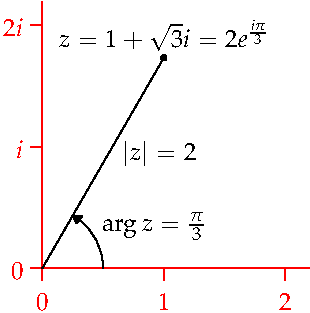
\includegraphics{binary-polar}
\end{minipage}\\

The polar form is nothing more than using standard polar co-ordinates to describe points on the Argand diagram. The primary non-trivial aspect of this is the \emph{complex exponential,} which may be computed using \emph{Euler's formula}:\footnote{More generally, $e^{x+iy}=e^xe^{iy}=e^x\cos y+ie^x\sin y$. To prove Euler's formula, one can either use differential equations or Maclaruin series (after assuming that these make sense for complex numbers).}
\[e^{i\theta}=\cos\theta+i\sin\theta\]
which is the source of the famous identity $\displaystyle e^{i\pi}=-1$. A quick computation with the polar form allows one to check the following:

\begin{lemm}
Suppose that $z,w\in\C$. Then
\begin{itemize}
  \item $\nm{zw}=\nm z\nm w$.
  \item $\arg(zw)=\arg(z)+\arg(w)$ (perhaps after subtracting $2\pi$).
\end{itemize}
\end{lemm}

% Arguably the most useful fact regarding the complex numbers is the following result.
% \begin{thm}[Fundamental Theorem of Algebra]
% If $p(z)=a_nz^n+a_{n-1}z^{n-1}+\cdots+a_1z+a_0$ is a degree $n$ polynomial ($a_n\neq 0$), then the equation $p(z)=0$ has exactly $n$ roots over the complex numbers. Otherwise said, there exist exactly $n$ complex numbers $\lst zn$ such that
% \[p(z)=a_n(z-z_1)(z-z_2)\cdots (z-z_n)\]
% \end{thm}

\begin{defn}
Let $n\in\N_{\ge 2}$. The $n^\text{th}$ roots of unity\footnote{In this context, \emph{unity} is simply a pretentious term for the number 1.} are the (complex) solutions to the equation $z^n=1$.
\end{defn}

For example, the square-roots of unity are $\pm 1$. Thanks to the fundamental theorem nad Euler's formula, we can easily describe the $n^\text{th}$ roots.

\begin{thm}
Suppose that $n$ is fixed and let $\zeta=e^{\frac{2\pi i}n}$. Then the $n^\text{th}$ roots of unity are precisely the values
\[1,\zeta,\zeta^2,\cdots,\zeta^{n-1}\]
\end{thm}

\begin{proof}
We find all the solutions to the equation $z^n=1$. Take the modulus of both sides to obtain $\nm{z}^n=1$. Since $\nm{z}$ is a positive real number (it certainly can't be zero!), the only solution is $\nm{z}=1$. The polar form is therefore $z=e^{i\theta}$. Now compute:
\[1=z^n=(e^{i\theta})^n=e^{in\theta}\iff n\theta=2\pi k\]
for some integer $k$. Thus $\theta=\frac{2\pi k}n$ and so
\[z=e^{i\theta}=e^{\frac{2\pi i}nk}=\left(e^{\frac{2\pi i}n}\right)^k=\zeta^k\tag*{\qedhere}\]
\end{proof}

The $n^\text{th}$ roots are equally spaced around the unit circle, forming the corners of a regular $n$-gon centered at the origin, with one corner at 1.

\begin{center}
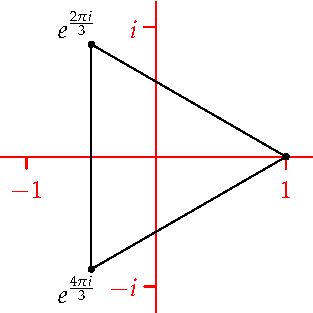
\includegraphics{binary-rootunity2}
\qquad\qquad\qquad
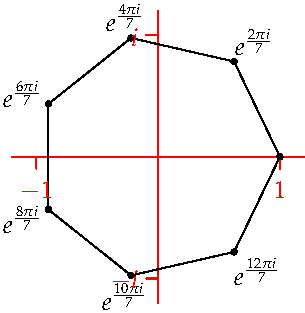
\includegraphics{binary-rootunity}
\end{center}

Why are we interested in the $n^\text{th}$ roots? Because they are \emph{closed under multiplication}: $\displaystyle\zeta^k\cdot\zeta^l=\zeta^{k+l}$.


\section{Morphisms}\label{sec:morph}

One of the purposes of abstract algebra is to observe and describe common structure. Mathematicians do this by defining functions: a \emph{morphism} is a function which preserves some structure. The type of structure preserved depends on the context. In this course, all morphisms will have one of the prefixes \emph{homo} or \emph{iso}. These mean, respectively, \emph{similar} and \emph{same}.

\begin{defn}\label{defn:homo}
Let $X,Y$ be sets with binary operations $*_X,*_Y$. A function\footnote{If the binary structures are known to the reader, one typically just writes $\phi:X\to Y$.} $\phi:(X,*_X)\to(Y,*_Y)$ is:
\begin{itemize}
  \item A \emph{homomorphism} if $\displaystyle\forall a,b\in X,\quad \phi(a*_Xb)=\phi(a)*_Y\phi(b)$.
  \item An \emph{isomorphism} if is a bijective\footnote{Recall the definitions: A function $f:X\to Y$ is said to be;
	\begin{itemize}
		\item \emph{injective/1--1} if $f(x)=f(y)\implies x=y\text{ for all }x,y\in X$.
		\item \emph{surjective/onto} if $\operatorname{range}(f)=Y$.
		\item \emph{bijective} if it is both injective and surjective.
	\end{itemize}} homomorphism.
\end{itemize}
If there exists an isomorphism $\phi$, we say that $(X,*_X)$ and $(Y,*_Y)$ are \emph{isomorphic binary structures,}\footnote{If two structures are isomorphic, there likely exist several different isomorphisms. There are alternative notations for when you want to stress the particular isomorphism, for instance $\phi:X\cong Y$ or $\phi:X\!\! \begin{array}{c} \sim\\[-2ex]\longrightarrow\\[-2ex]- \end{array} \!\!Y$.} and write $X\cong Y$.
\end{defn}




\paragraph{Examples}
\begin{enumerate}
  \item Let $\phi:\Z\to\Z$ be the function $\phi(x)=2x$. Then
  \[\phi(x+y)=2(x+y)=2x+2y=\phi(x)+\phi(y)\]
  so that $\phi$ is a homomorphism. This function is not an isomorphism, since it is not surjective.
  \item If $V,W$ are vector spaces and $L:V\to W$ is a linear map then $L$ is a homomorphism for the binary structures of vector addition.
  \item Revisit the \hyperlink{sec:motiv}{motivational example} for an in-depth example of an isomorphism of binary structures $S_3\cong D_3$.
  \item The function $\phi:(\R,+)\to(\R^+,\cdot)$ defined by $\phi(x)=e^x$ is an isomorphism. It is certainly bijective, and the exponential laws tell us that
  \[\phi(x+y)=e^{x+y}=e^xe^y=\phi(x)\phi(y)\]
  Indeed $\psi(z)=e^z$ is a \emph{homomorphism} $\psi:(\C,+)\to(\C,\cdot)$. You should be able to give \emph{at least two} reasons why $\psi$ is not an isomorphism!
  \item The function $\phi:(\R,+)\to (\C,\cdot)$ defined by $\phi(x)=e^{ix}$ is a homomorphism.
  \item The set $\{0,1,2\}$ under addition modulo 3 and the cube-roots of unity $\{1,\zeta,\zeta^2\}$ under multiplication have tables
	\[\begin{array}{c||c|c|c}
	+_3 & 0 & 1 & 2 \\
	\hline\hline 1 & 0 & 1 & 2\\
	\hline 1 & 1 & 2 & 0\\
	\hline 2 & 2 & 0 & 1
	\end{array}
	\qquad\qquad 
	\begin{array}{c||c|c|c}
		\cdot & 1 & \zeta & \zeta^2 \\
		\hline\hline 1 & 1 & \zeta & \zeta^2\\
		\hline \zeta & \zeta & \zeta^2 & 1\\
		\hline \zeta^2 & \zeta^2 & 1 & \zeta
  \end{array}\]
	The function
	\[\phi:\{0,1,2\}\to\{1,\zeta,\zeta^2\}:x\mapsto \zeta^x\]
	is an isomorphism of binary structures. You should think carefully on the commonality between examples 4, 5 and 6\ldots
\end{enumerate}

\subsubsection*{Pull-backs}

It is very easy to create examples of isomorphic binary structures. Given a \emph{bijection} $\phi:X\to Y$ and a binary operation $\star$ on $Y$, you can always define an operation $*$ on $X$ by \emph{pulling-back} $\star$ to $X$:
\[x_1\,*\,x_2:=\phi^{-1}(\phi(x_1)\star\phi(x_2))\]


\begin{enumerate}
  \item The map $\phi:\R^+\to\R^+:x\mapsto x^2$ is a bijection. Suppose we want $\phi$ to be an isomorphism $\phi:(\R^+,*)\to(\R^+,+)$. Then we must define $*$ by
	\[x*y:=\phi^{-1}(\phi(x)+\phi(y))=\phi^{-1}(x^2+y^2)=\sqrt{x^2+y^2}\]
	\item Now suppose that we want $\phi$ to be an isomorphism $\phi:(\R^+,+)\to(\R^+,\star)$. This time we must have $\phi$ satisfying
	\[\phi(x)\star\phi(y)=\phi(x+y)\implies x^2\star y^2=(x+y)^2\]
	The required binary operation is therefore $X\star Y=(\sqrt X+\sqrt Y)^2$.
\end{enumerate}


\subsection*{Showing Isomorphicity}

Often the challenge is to determine whether two structures $(X,*)$ and $(Y,\star)$ are isomorphic. The first step is to develop a gut feeling---this only comes with practice! If you think that the structures are isomorphic, then you should follow the steps below:
\begin{itemize}\renewcommand{\itemsep}{0cm}
  \item Define a function $\phi:X\to Y$,
  \item Check that $\phi$ is a homomorphism:\ \ $\phi(x*y)=\phi(x)\,\star\,\phi(y)$,
  \item Check $\phi$ is injective:\ \ $\phi(x)=\phi(y)\implies x=y$,
  \item Check $\phi$ is surjective:\ \ $\forall y\in Y,\ \exists x\in X$ such that $y=\phi(x)$.
\end{itemize}
You can perform the final three steps in any order you like. Sometimes it is easier to think of a bijection, then check that it is a homomorphism; other times it is easier to use the homomorphism property to choose a function, then check that you have a bijection.

\paragraph{Examples}
\begin{enumerate}
  \item Prove that $2\Z\cong 3\Z$ with the binary operation of addition on both sides.
  \begin{description}
      \item[Define $\phi$:] Let $\phi:2\Z\to 3\Z:2n\mapsto 3n$, i.e.\ $\phi(x)=\frac{3}{2}x$.
      \item[Homomorphism:] $\phi(x+y)=\frac{3}{2}(x+y)=\frac{3}{2}x+\frac{3}{2}y=\phi(x)+\phi(y)$.\ \ \checkmark
      \item[Injective:] $\phi(x)=\phi(y)\implies \frac{3}{2}x=\frac{3}{2}y\implies x=y$.\  \ \checkmark
      \item[Surjective:] An arbitrary element of $3\Z$ is $z=3m$ where $m\in\Z$. But $3m=\phi(2m)$.\ \ \checkmark
  \end{description}
  $\phi$ is therefore an isomorphism $\phi:2\Z\cong 3\Z$.
  \item The bijection $\phi(x)=\frac 32 x$ is also an isomorphism $2\Z\cong 3\Z$ with respect to the binary operations $x*y=\frac{1}{2}xy$ on $2\Z$ and $x\star y=\frac{1}{3}xy$ on $3\Z$.
\end{enumerate}

\subsection*{Showing non-isomorphicity}

On the face of it this is harder, as there is no general way to do this. Unless $X,Y$ are very small sets, you can't realistically test every function $X\to Y$. Instead we have to be a little more cunning.

\begin{defn}
A \emph{structural property} of $(X,*)$ is a property which is preserved under isomorphisms: i.e.\ if $\phi:(X,*)\to (Y,\star)$ is an isomorphism then $(X,*)$ and $(Y,\star)$ have the same structural properties.
\end{defn}

The following is a non-exhaustive list of structural properties: suppose $\phi:X\to Y$ is an isomorphism throughout.

\begin{description}
  \item[Cardinality] If $X\cong Y$, then the elements of $X,Y$ are bijectively paired, whence the cardinalities of $X$ and $Y$ are the same. This is true even for infinite sets: recall that $\nm\N=\nm\Q=\aleph_0\lneq \nm\R$, so there are \emph{no} isomorphisms between $\Q$ and $\R$, no matter what binary operations you have.
  \item[Commutativity \& Associativity] For instance if $(X,\ast)$ is commutative, then
  \[\forall a,b\in X,\ \phi(a)\star\phi(b)=\phi(a*b)=\phi(b*a)=\phi(b)\star\phi(a)\]
  Since $\phi$ is bijective, every element of $Y$ has the form $\phi(a)$ for some $a\in X$. Thus $(Y,\star)$ is commutative.
  \item[Identity] If $X$ has an identity element $e$ then $\phi(e)$ is an identity for $Y$.
  \item[Solutions to equations] An element $x\in X$ is \emph{idempotent} if $x*x=x$. It follows that $\phi(x)\star\phi(x)=\phi(x)$ in $Y$. Thus if idempotents exist in $X$, but do not in $Y$, there can be no isomorphism.\\
  More generally: if the equation $a*x=b$ has a solution $x\in X$, then the corresponding equation $\phi(a)\star\phi(x)=\phi(b)$ must have a solution $\phi(x)$ in $Y$.
\end{description}

There are many other possible structural properties. Indeed the more complex the structure, the more potential properties there are to consider. Disproving isomorphicity is somewhat of an art, requiring a flash of inspiration to find the correct structural property. It is also important to note that there are many concepts that are not necessarily preserved by an isomorphism: the type of element (a number, a matrix, etc.), the type of binary operation (e.g.\ addition versus multiplication).

\paragraph{Examples}
\begin{enumerate}
	\item The two binary operations defined by the multiplication tables on page \pageref{eq:commute} are non-isomorphic because the first is commutative while the second is not.
	\item $(\R^3,+)\ncong(\R^3,\times)$ (cross product), because $+$ is commutative and associative, while $\times$ is neither.
	\item $(\N_0,+)\ncong(\N,+)$ since $\N_0$ contains an identity element 0 while $\N$ does not.
	\item $(\Q,+)\ncong(\Q^+,\cdot)$ since $y^2=2$ has no solution in $\Q$, but the corresponding equation $x+x=c$ has a solution for any $c\in\Q$.
\end{enumerate}



